\documentclass[spanish,12pt,letterpaper]{article}

\usepackage[margin=0.5in]{geometry}
\usepackage[spanish]{babel}
\usepackage[utf8]{inputenc}
\usepackage{authblk}
\usepackage{amsmath}
\usepackage{amssymb}
\usepackage{graphicx}

\title{Análisis de Algoritmos\\ Práctica 2: Ordenamientos}
\author{López García Gilberto Isaac}
\affil{Facultad de Ciencias, UNAM}
\date{Lunes 31 de octubre de 2016}

\begin{document}

\maketitle

\section{Tiempos de ejecución}

\subsection{Mejor caso}

Comparación de tiempos para el mejor caso de \textsc{Quick Sort}, \textsc{Merge Sort} y \textsc{Bubble Sort} para tamaños de ejemplar de 10 hasta 5,000.

{
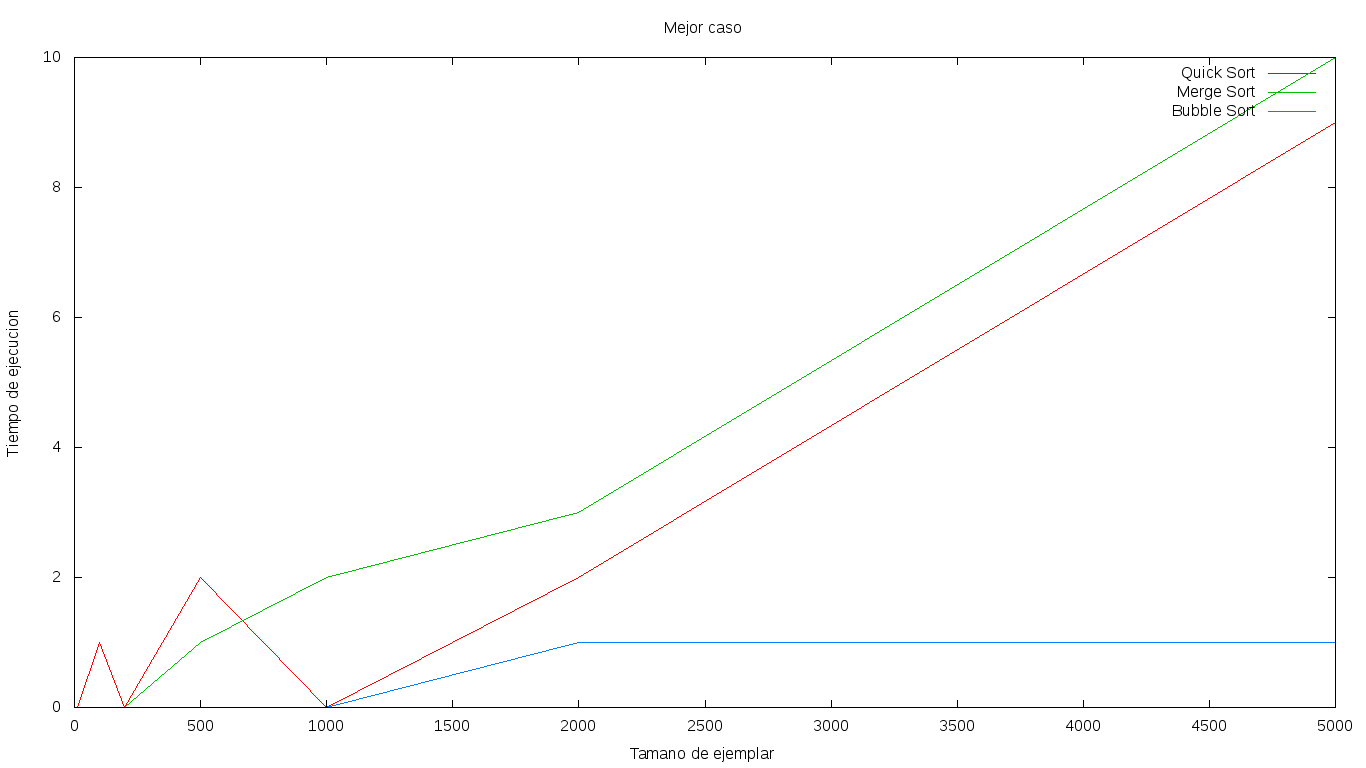
\includegraphics[scale=0.5]{mejorcaso_5m}
\centering
}

\newpage
Comparación de tiempos para el mejor caso de \textsc{Quick Sort}, \textsc{Merge Sort} y \textsc{Bubble Sort} para tamaños de ejemplar de 10 hasta 500,000.

{
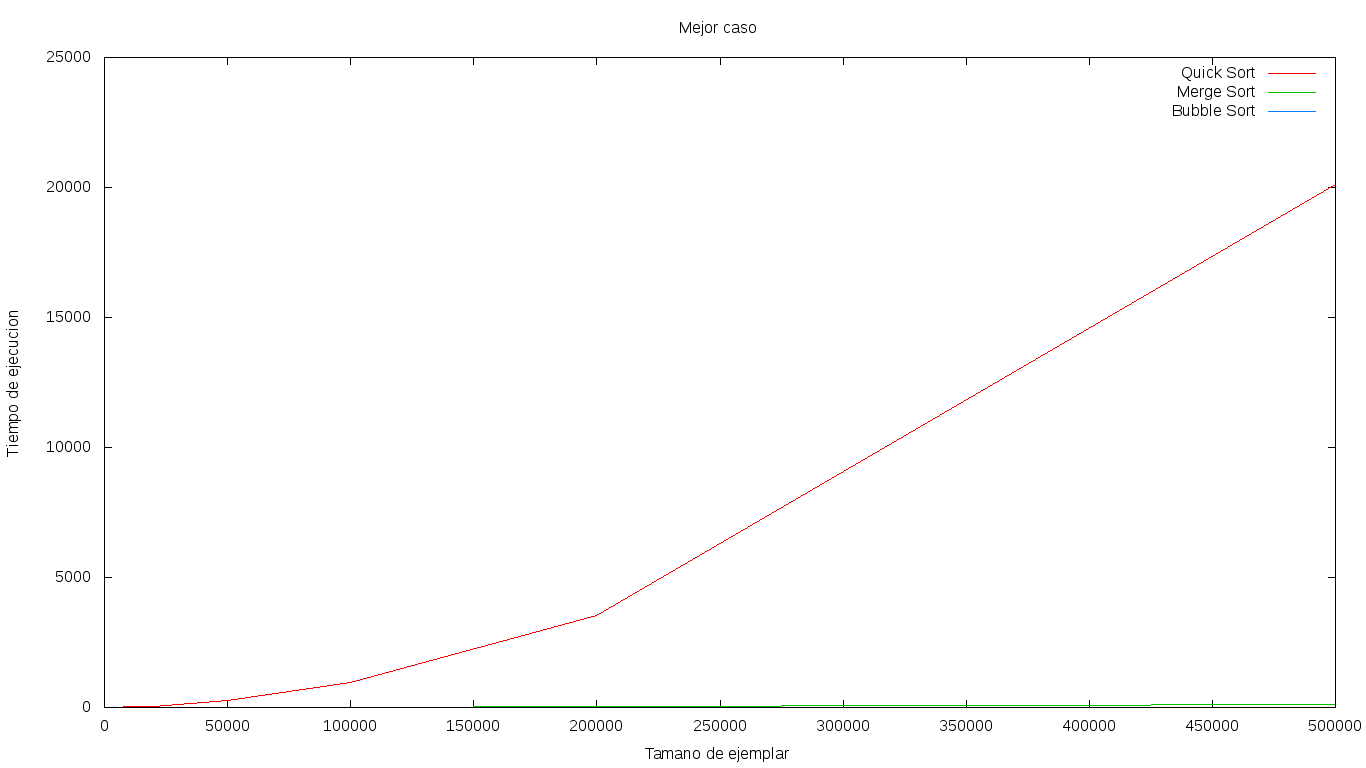
\includegraphics[scale=0.5]{mejorcaso_500m}
\centering
}

\subsection{Peor caso}

Comparación de tiempos para el peor caso de \textsc{Quick Sort}, \textsc{Merge Sort} y \textsc{Bubble Sort} para tamaños de ejemplar de 10 hasta 5,000.

{
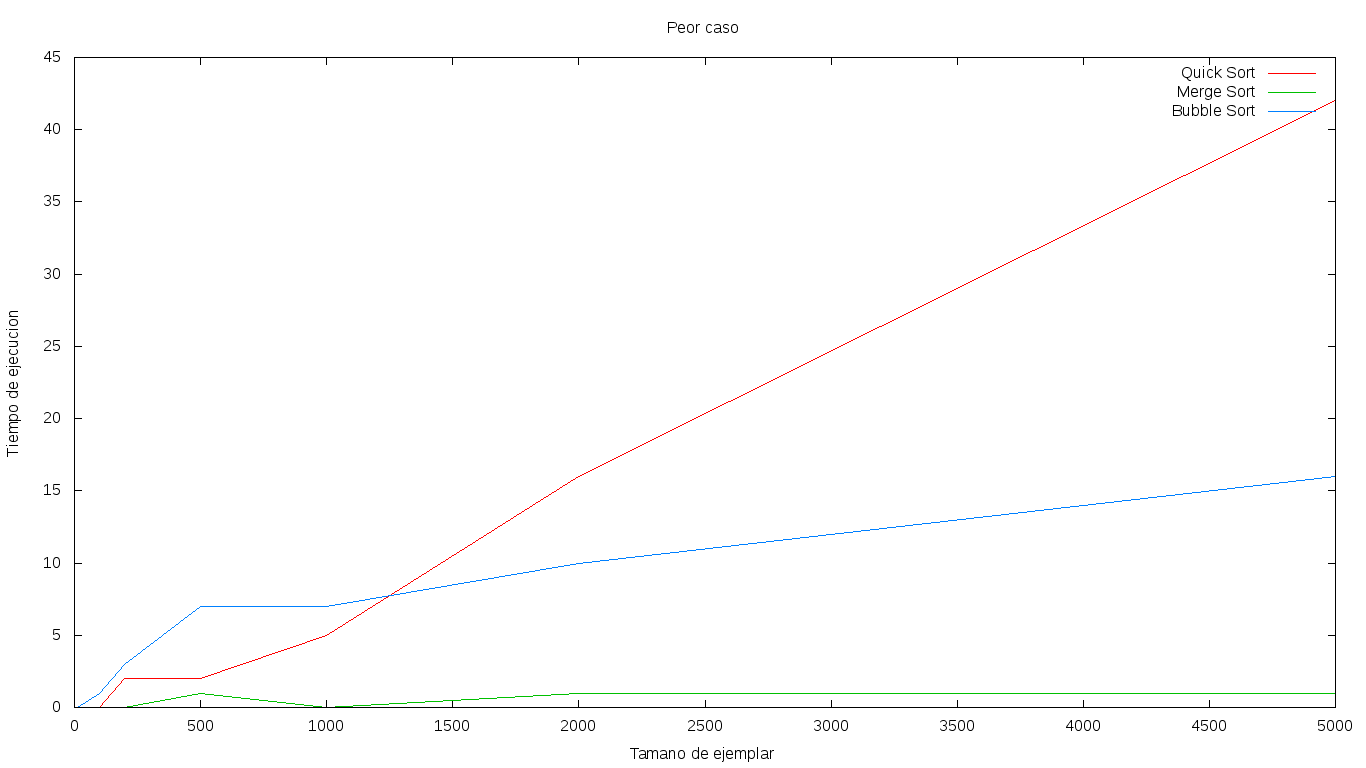
\includegraphics[scale=0.5]{peorcaso_5m}
\centering
}

\newpage
Comparación de tiempos para el peor caso de \textsc{Quick Sort}, \textsc{Merge Sort} y \textsc{Bubble Sort} para tamaños de ejemplar de 10 hasta 500,000.

{
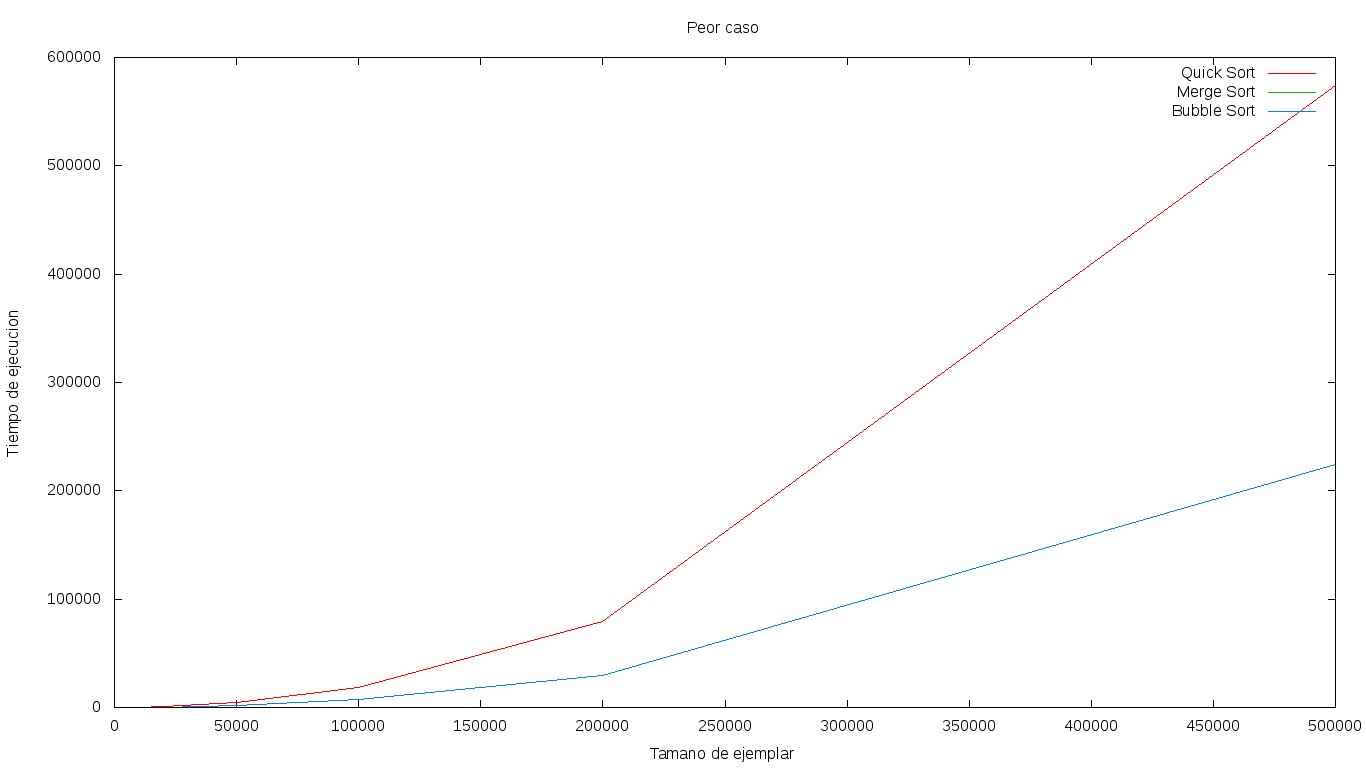
\includegraphics[scale=0.5]{peorcaso_500m}
\centering
}

\subsection{Tiempos de Quick Sort}

Comparación de tiempos del peor caso de \textsc{Quick Sort} contra el peor caso.

{
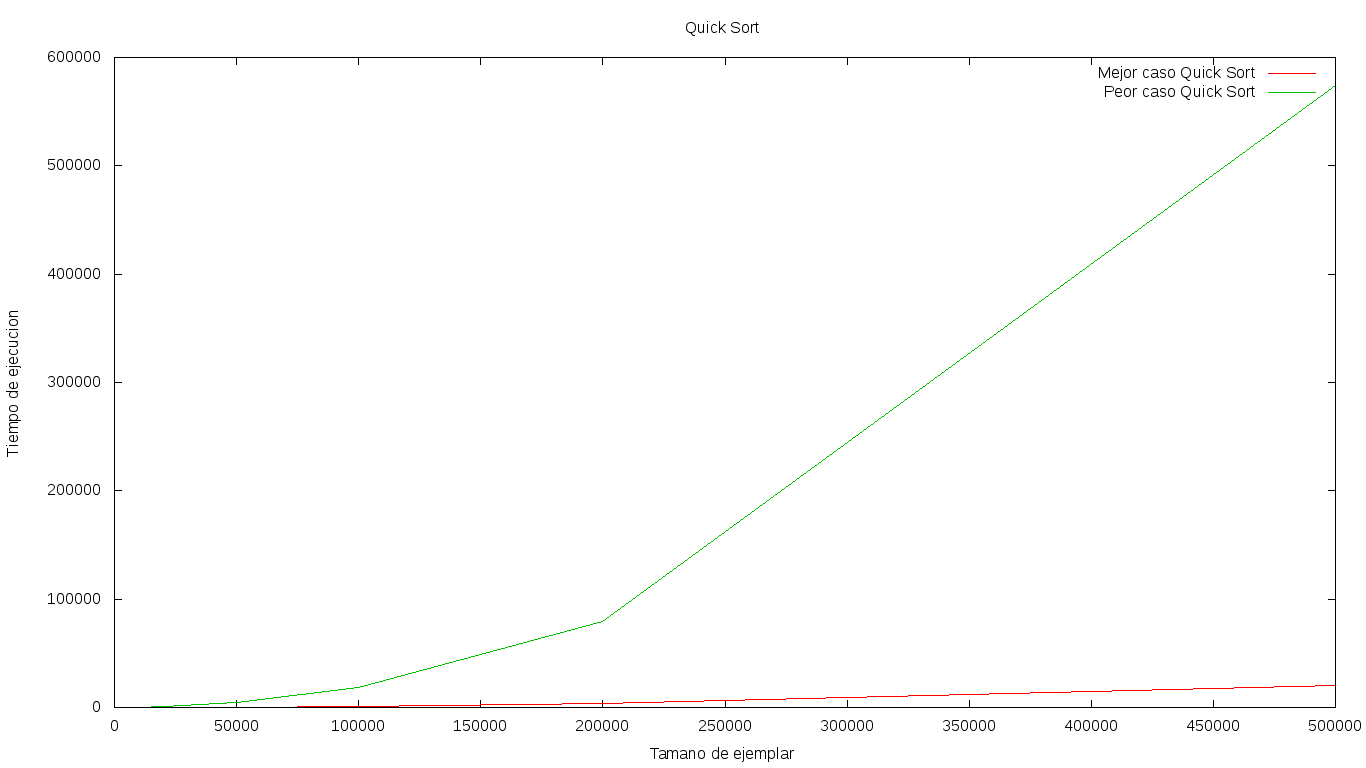
\includegraphics[scale=0.5]{quickSort}
\centering
}

\subsection{Tiempos de Merge Sort}

Comparación de tiempos del peor caso de \textsc{Merge Sort} contra el peor caso.

{
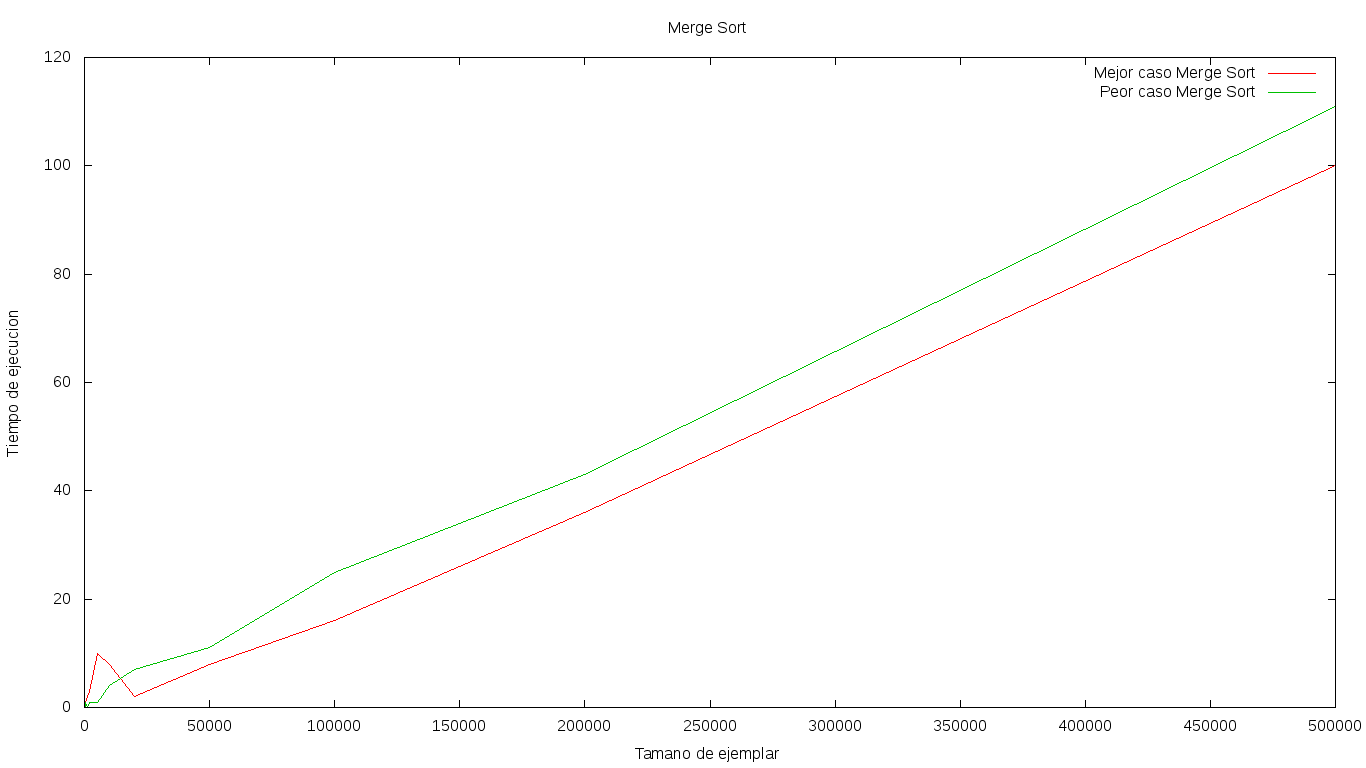
\includegraphics[scale=0.5]{mergeSort}
\centering
}

\subsection{Tiempos de Bubble Sort}

Comparación de tiempos del peor caso de \textsc{Bubble Sort} contra el peor caso.

{
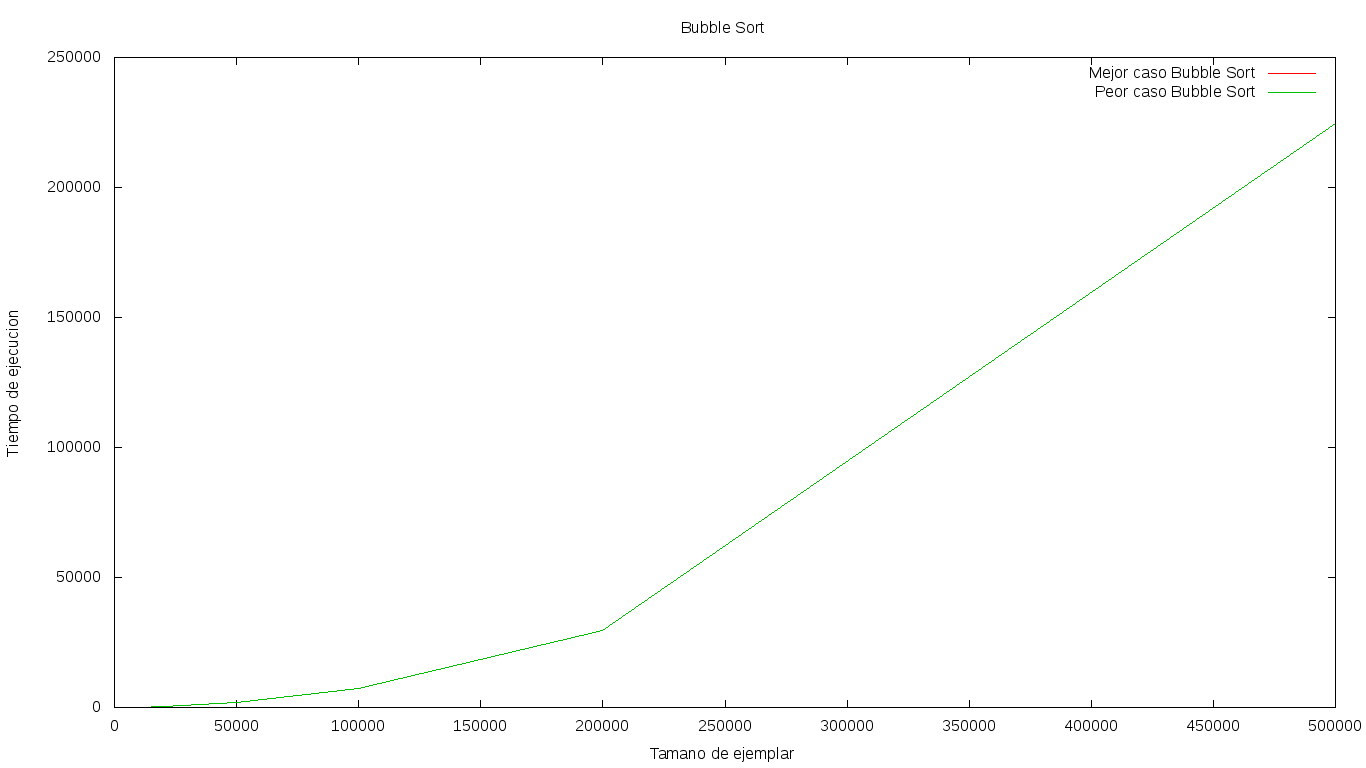
\includegraphics[scale=0.5]{bubbleSort}
\centering
}

\end{document}
